\documentclass{article}
\usepackage[a4paper,margin=1in]{geometry}
\usepackage{graphicx}
\graphicspath{ {images/} }
\usepackage[utf8]{inputenc}
\usepackage{minted}
\usepackage[brazilian]{babel}

\newenvironment{pycode}[2][h!]
 {\VerbatimEnvironment
  \begin{minted}[frame=single,framesep=3mm,label=Python: #2,breaklines=true]{python}}
 {\end{minted}}

 
 \newenvironment{rcode}[2][h!]
 {\VerbatimEnvironment
  \begin{minted}[frame=single,framesep=3mm,label=R: #2,breaklines=true]{R}}
 {\end{minted}}

\title{Métodos Quantitativos}
\author{Marcos Rodrigues, Matheus Alcântara, Pedro Ruas}
\date{Maio 2017}

\begin{document}

\maketitle

\section{Introdução}

Este documento apresenta uma relação de códigos e procedimentos implementados, utilizando as linguagens Python e R, tal como a ferramenta \emph{Minitab Express}, para explorar as técnicas dentro do contexto de Métodos Quantitativos em Ciência da Computação.

Para a linguagem Python, foram utilizadas bibliotecas que implementam os cálculos e operações necessárias, sendo elas a biblioteca NumPy (incluindo o pacote Linalg) e SKLearn.
A linguagem R contempla em suas bibliotecas as operações necessárias para o desenvolvimento dos códigos aqui descritos.


\section{Revisão de matrizes}

Neste capítulo demonstramos exemplos de implementações que efetuam operações em matrizes. Para exemplo, foram geradas matrizes aleatórias de tamanho $5x5$, composta de inteiros variando de $-9$ a $10$. Para a geração das matrizes de números aleatórios, utilizamos os códigos que seguem. Considere $m1$, $m2$, $A$ e $B$ como as matrizes utilizadas nos exemplos.

\begin{pycode}{Revisão de matrizes}
# Importa a biblioteca NumPy para uso 
import numpy as np

# Gerar matrizes aleatórias
m1 = np.random.randint(-9, 10, size=(5, 5))
m2 = np.random.randint(-9, 10, size=(5, 5))

# A seguir, uma série de operações que podem ser realizadas utilizando matrizes, em códigos usando Python e R

#Soma algébrica
soma = np.add(m1, m2) # Entre duas matrizes
soma = np.add(4, m1)  # Entre um escalar e uma matriz

# Multiplicação
mult =  np.matmul(m1, m2)   # m1 x m2
mult =  np.matmul(m2, m1)   # m2 x m1
mult =  np.matmul(m1,  4)   # m1 x 4, um escalar

#Triangular superior e inferior
superior = np.triu(m1)
inferior = np.tril(m1)

#Diagonal
diag = np.diag(m1)

#Identidade
identidade=np.identity(5)

#Transposta e simétrica
transposta = np.matrix.transpose(m1)
isSimetrica = np.array_equal(m1,transposta)  # Verifica se a matriz é simétrica

#Inversa
inversa = np.linalg.inv(m1)

#Determinante
determinante = np.linalg.det(m1)

#Adjunta (adjunta = determinante * inversa)
adjunta = np.linalg.det(m1) * np.linalg.inv(m1)

#Menor complementar
def menorComp(matriz, i, j):
	# Função: retira a linha e coluna (i,j) e retorna o determinante
	temp = np.delete(np.delete(matriz, j, 1), i, 0)
	return np.linalg.det(temp)
# Menor complementar da linha 1 e coluna 2
minor = menorComp(m1, 1, 2)) 

#Matriz de cofatores
def matrizDeCofatores(matriz):
	# Para cada elemento, calcular o menor complementar (determinante removendo a linha e coluna)
	# Em cada valor obtido, multiplicar por ((-1)**(i+j)))
	temp = np.full_like(matriz, 0)
	for index in np.ndindex(matriz.shape):
		i,j = (index)
		temp[index] = ((-1)**(i+j)) * menorComp(matriz, i, j)
	return temp
cofatores = matrizDeCofatores(m1)

#Posto ou Rank
rank = np.linalg.matrix_rank(m1)

#Autovalor e autovetor
autovalor, autovetor = np.linalg.eig(m1)

#Equações lineares
# Exemplo:
#   x – y – z + w = 10
#   2x + 3y + 5z – 2w = 21
#   4x – 2y – z + w = 16
coeficientes = np.array([[ 1,-1,-1, 1],
						 [ 2, 3, 5,-2],
						 [ 4,-2,-1, 1]])
valores = np.array([10,21,16])

# Este método requer uma matrix quadrática
resultado = np.linalg.solve(coeficientes, valores) 

# Método 'least-squares-fitting', que minimiza o erro da solução aproximada
resultado = np.linalg.lstsq(coeficientes, valores)
\end{pycode}

\begin{rcode}{Revisão de matrizes}
# Gerar matrizes aleatórias
A <- matrix(sample(-9:10,15), nrow=5, ncol=5)
B <- matrix(sample(-9:10,15), nrow=5, ncol=5)

#Soma algébrica
cat("Soma (A+B):\n") ; A+B

# Multiplicação
A ; 3*A             # Multiplicação por um escalar
A ; B ; A*B         # Multiplicação dos elementos das matrizes
A ; B ; A %*% B   # Multiplicação das matrizes

# Triangular superior e inferior
SUPERIOR <- upper.tri(A, diag=TRUE)
INFERIOR <- lower.tri(A, diag=TRUE)

# Diagonal
D <- diag(A)

# Identidade
I <- diag(1,nrow=dim(A)[1]) # Matriz identidade

# Transposta e simétrica
TRANSPOSTA <- t(A)
isSimetrica - isSymmetric.matrix(A)

# Inversa
INV <- solve(A)

# Determinante
DET <- det(A)
DET <- det(t(A)) # Determinante da transposta de A

# Adjunta (adjunta = determinante * inversa)
ADJ <- det(A) * solve(A)

# Matriz de cofatores
A <- matrix(data=c(1, 2, 3, 2, 5, 9, 5, 7, 8), nrow=3, ncol=3)
minor <- function(A, i, j) det( A[-i,-j] )
cofactor <- function(A, i, j) (-1)^(i+j) * minor(A,i,j)
adjoint1 <- function(A) { #Loop
  n <- nrow(A)
  B <- matrix(NA, n, n)
  for( i in 1:n )
    for( j in 1:n )
      B[j,i] <- cofactor(A, i, j)
  B
}

adjoint2 <- function(A) { #Outer
  n <- nrow(A)
  t(outer(1:n, 1:n, Vectorize(
    function(i,j) cofactor(A,i,j)
  )))
}
cat("Cofator da matriz A:\n") ; A %*% adjoint1(A)
cat("Cofator da matriz A:\n") ; A %*% adjoint2(A)

# Posto ou Rank
POSTO <- matrix(rank(A), nrow=length(A[,1]), ncol=length(A[1,]))

# Autovalor e autovetor
A <- matrix(c(3,-1,1,-1,5,-1,1,-1,3), nrow=3, ncol=3)
y <- eigen(A)
cat("Autovalores da matriz A:\n") ; y$values
cat("Autovetores da matriz A:\n") ; round(y$vectors)

# Equações lineares
A <- matrix(data=c(1, 2, 3, 2, 5, 9, 5, 7, 8), nrow=3, ncol=3, byrow=TRUE)    
x <- matrix(data=c(20, 100, 200), nrow=3, ncol=1, byrow=FALSE)
b <- round(solve(A, x), 3) ; rownames(b) <- c("x","y","z")
cat("Sistema de equacoes [A][x]=[y]\n") 
cat("Matriz A:\n") ; A 
cat("Matriz x:\n") ; x
cat("Matriz solucao b:\n") ; b
\end{rcode}
    
    


\section{Análise de Componentes Principais}

Neste capítulo demonstramos exemplos de implementações envolvidas na Análise de Componentes Principais, ou em inglês \textit{Principal Component Analysis (PCA)}. Para tanto, fizemos o uso da biblioteca SKLEARN em Python, com o módulo PCA. Em R, as funções já estão nativamente implementadas.

\begin{pycode}{Análise de Componentes Principais}
# Importa a biblioteca NumPy e as funções de PCA da biblioteca SKLEARN  
import numpy as np
from sklearn.decomposition import PCA

# Gera uma matriz aleatória
X = np.random.randint(0, 10, size=(7, 7))

# Inicia o PCA, sobre a matriz X
pca = PCA(n_components=5)   
pca.fit(X)

# Exibe as principais componentes, representando as direções de variância máxima nos dados. As componentes são ordenadas pela variância explicada
print (pca.components_)
        
# Exibe a variância explicada de cada componente selecionado
print(pca.explained_variance_) 

# Exibe o percentual de variância explicada por componente
print(pca.explained_variance_ratio_) 

# Exibe a variância explicada acumulada
print(pca.explained_variance_ratio_.sum()) 

# Realiza a redução de dimensionalidade na matriz X
print(pca.transform(X))
\end{pycode}

\begin{rcode}{Análise de Componentes Principais}
data(decathlon2)

# Extrai os indivíduos ativos e as variáveis para a PCA
decathlon2.active <- decathlon2[1:23, 1:10]
head(decathlon2.active[, 1:6])
res.pca <- prcomp(decathlon2.active, scale=TRUE)

# res.pca, extraídos da função prcomp, são os valores, e podem ser exibidos com este comando
names(res.pca)
print(res.pca)

# Os desvios padrões dos componentes principais (raiz quadrada dos autovalores)
head(res.pca$sdev)
  
# A matriz com os pesos das variáveis (as colunas são os autovetores)
head(unclass(res.pca$rotation)[, 1:4])

# Autovalores
eig <- (res.pca$sdev)^2
# Variâncias, em %
variance <- eig*100/sum(eig)
# Variâncias acumuladas
cumvar <- cumsum(variance)
eig.decathlon2.active <- data.frame(eig=eig, variance=variance, cumvariance=cumvar)
head(eig.decathlon2.active)

summary(res.pca)        
fviz_screeplot(res.pca, ncp=10)
head(res.pca)
fviz_pca_var(res.pca)
fviz_pca_var(res.pca, col.var="cos2") +
  scale_color_gradient2(low="white", mid="blue", 
                        high="red", midpoint=0.5) + theme_minimal()

# Contribuição das variáveis na primeira componente
fviz_pca_contrib(res.pca, choice = "var", axes = 1)
fviz_pca_contrib(res.pca, choice = "var", axes = 1, top = 7)

# Contribuição das variáveis na segunda componente
fviz_pca_contrib(res.pca, choice = "var", axes = 2)

# Contribuição na primeira e segunda componentes
fviz_pca_contrib(res.pca, choice = "var", axes = 1:2)
\end{rcode}
    
    

\section{Decomposição em Valores Singulares}

Neste capítulo demonstramos exemplos de implementações envolvidas na Decomposição em Valores Singulares, ou em inglês \textit{Singular Value Decomposition (SVD)}. Também fizemos o uso da bilbioteca SKLEARN em Python. Da mesma forma que em PCA, as funções já estão nativamente implementadas em na linguagem R.

\begin{pycode}{Decomposição em Valores Singulares}
# Importa a biblioteca NumPy e as funções de SVD da biblioteca SKLEARN para uso 
import numpy as np
from sklearn.decomposition import TruncatedSVD

# Gera uma matriz aleatória
X = np.random.randint(0, 10, size=(7, 7))

# Inicia a operação de SVD sobre a matriz X e exibe as componentes
svd = TruncatedSVD(n_components=5, n_iter=7, random_state=20)
svd.fit(X)
print (svd.components_)

# Exibe a variância dos dados de treinamento, transofrmados por uma projeção de cada componente
print(svd.explained_variance_) 

# Exibe o percentual de variância explicada por componente
print(svd.explained_variance_ratio_) 

# Exibe a variação explicada acumulada
print(svd.explained_variance_ratio_.sum()) 

# Realiza a redução de dimensionalidade na matriz X
print(svd.transform(X))
\end{pycode}

\begin{rcode}{Decomposição em Valores Singulares}
# A linha abaixo importa um conjunto de dados da URL fornecida 
cnut <- read.dta("http://statistics.ats.ucla.edu/stat/data/cerealnut.dta")

# Centralizando as variáveis
mds.data <- as.matrix(sweep(cnut[, -1], 2, colMeans(cnut[, -1])))
dismat <- dist(mds.data)
mds.m1 <- cmdscale(dismat, k = 8, eig = TRUE)
mds.m1$eig

mds.m1 <- cmdscale(dismat, k = 2, eig = TRUE)
x <- mds.m1$points[, 1]
y <- mds.m1$points[, 2]
plot(x, y)
text(x + 20, y, label=cnut$brand)

# Autovalores
xx <- svd(mds.data %*% t(mds.data))
xx$d

# Coordenadas
xxd <- xx$v %*% sqrt(diag(xx$d))
x1 <- xxd[, 1]
y1 <- xxd[, 2]

# Para plotar os valores, mostrando o gráfico
plot(x1, y1)
text(x1 + 20, y1, label=cnut$brand)
\end{rcode}
    
    
\section{Análise Fatorial}

Neste capítulo demonstramos exemplos de implementações envolvidas na Decomposição em Valores Singulares, ou em inglês \textit{Singular Value Decomposition (SVD)}. Também fizemos o uso da bilbioteca SKLEARN em Python. Da mesma forma que em PCA, as funções já estão nativamente implementadas em na linguagem R.

\begin{pycode}{Análise Fatorial}
# Importa a biblioteca NumPy e as funções de Análise Fatorial da biblioteca SKLEARN para uso 
import numpy as np
from sklearn.decomposition import FactorAnalysis

# Gera uma matriz aleatória
X = np.random.randint(0, 10, size=(7, 7))

# Inicia a operação de Análise Fatorial sobre a matriz X e exibe as componentes
fa = FactorAnalysis(n_components=5)
fa.fit(X)
print (fa.components_)

# Calcula a covariância dos dados com o modelo de Análise Fatorial
print (fa.get_covariance())

# Exibe probabilidade logarítmica em cada iteração da Análise Fatorial
print(fa.loglike_) 

# Exibe variância do ruído estimado para cada feature
print(fa.noise_variance_) 

# Calcula a probabilidade logarítmica média das amostras (scores)
print(fa.score(X))

# Realiza a redução de dimensionalidade na matriz X
print(fa.transform(X))
\end{pycode}

\begin{rcode}{Análise Fatorial}
# Importa bibliotecas necessárias e bases de teste disponíveis no R
install.packages("psych")
library(psych)
require(foreign)
library( GPArotation )

# Inicia os dados de teste
data(bfi)
head(bfi)
describe(bfi)

# Faz a análise fatorial nos dados
df <- bfi[1:25]
scree(df)
fa.parallel(bfi)

# Exibe os resultados e plota o diagrama para consulta
out <- fa(df,6,fm='minres',rotate='oblimin')
print(out$loadings,cut=.2)
fa.diagram( out )
out <- fa(df,5,fm='minres','oblimin')
print(out$loadings,cut=.2)
fa.diagram( out )
\end{rcode}
    
    
    
\section{Regressão Linear Simples e Multipla}

Neste capítulo demonstramos exemplos de implementações relacionadas a Regressão Linear, simples ou multipla, e também a Função Logística. Novamente, fizemos o uso das bibliotecas NumPy e SKLEARN em Python, enquanto na linguagem R há implementação nativa. Adicionalmente, em Python, usamos a biblioteca MatPlot para plotar gráficos para melhor visualização dos resultados da regressão linear.

\begin{pycode}{Regressão Linear Simples}
# Importa as bibliotecas usadas.
# Note que a SKLEARN disponibiliza um módulo datasets, com bases de dados de exemplos
import matplotlib.pyplot as plt
import numpy as np
from sklearn import datasets, linear_model

# Carrega a base de testes relacionada à diabetes
diabetes = datasets.load_diabetes()

# Usar somente uma feature da base
diabetes_X = diabetes.data[:, np.newaxis, 2]

# Divide os dados em 2 conjuntos distintos: treinamento e testes
diabetes_X_train = diabetes_X[:-20]
diabetes_X_test = diabetes_X[-20:]

# Divide os alvos em 2 conjuntos distintos: treinamento e testes
diabetes_y_train = diabetes.target[:-20]
diabetes_y_test = diabetes.target[-20:]

# Inicia um objeto para fazer a regressão linear
regr = linear_model.LinearRegression()

# Treina o modelo de regressão usando a base de treinamento
regr.fit(diabetes_X_train, diabetes_y_train)

# Exibe os coeficientes calculados
print('Coeficientes: \n', regr.coef_)

# Exibe o coeficiente R2 da predição
print('R2: \n', diabetes_X_test,diabetes_y_test)

# Exibe o erro quadrático médio
print("Erro médior: %.2f"
      % np.mean((regr.predict(diabetes_X_test) - diabetes_y_test) ** 2))

# Exibe o score da variância explicada: 1 significa predição perfeita
print('Score: %.2f' % regr.score(diabetes_X_test, diabetes_y_test))

# Exibe a predição usando o modelo linear
print('Predição: \n', regr.predict(diabetes_X))

# Exibe o gráfico para visualização
plt.scatter(diabetes_X_test, diabetes_y_test,  color='black')
plt.plot(diabetes_X_test, regr.predict(diabetes_X_test), color='blue',
         linewidth=3)
plt.xticks(())
plt.yticks(())
plt.show()
\end{pycode}

\begin{rcode}{Regressão Linear Simples}
# Utiliza a base de dados Galapagos
galap <- read.table("https://sites.google.com/site/vllandeiror/dados/galapagos.txt", sep=" ", header=TRUE, quote="\"", colClasses="character", fileEncoding="UTF-8")
riqueza <- scan(text=galap[,3], dec=".")
area <- scan(text=galap[,2], dec=".")
plot(area,riqueza)

# Note que a relação não é linear e que um ponto assemelha-se a um outlier. Para linearizar os dados e reduzir o efeito do outlier tranformamos os dados em log.
riqueza.log <-log10(strtoi(riqueza,base=10))
area.log <- log10(as.double(area))
plot(area.log, riqueza.log) 

# Fazendo a regressão e mostrando os coeficientes a (intercepto) e b (inclinação) da regressão
resultado<-lm(riqueza.log ~ area.log)
resultado

# Detalhamento da regressão
summary(resultado) 

# Estatísticas: valores de t, probabilidades, os graus de liberdade e R2
summary.aov(resultado) 

# Gráficos para visualização, com a linha de tendência da regressão
plot(area.log,riqueza.log) 
abline(resultado)
\end{rcode}


\begin{pycode}{Regressão Linear Múltipla}
# Imports
import matplotlib.pyplot as plt
import numpy as np
from sklearn import datasets, linear_model

# Função Logística
# O conjunto de dados de teste é uma linha, com alguns ruídos gaussianos
xmin, xmax = -5, 5
n_samples = 100
np.random.seed(0)
X = np.random.normal(size=n_samples)
y = (X > 0).astype(np.float)
X[X > 0] *= 4
X += .3 * np.random.normal(size=n_samples)
X = X[:, np.newaxis]

# Classificar
clf = linear_model.LogisticRegression(C=1e5)
clf.fit(X, y)

# Gerando alguns gráficos para visualização
plt.figure(1, figsize=(7, 6))
plt.clf()
plt.scatter(X.ravel(), y, color='black', zorder=20)
X_test = np.linspace(-5, 10, 300)

# Mais gráficos relacionados à Regressão com Função Logística
def model(x):
    return 1 / (1 + np.exp(-x))
loss = model(X_test * clf.coef_ + clf.intercept_).ravel()
plt.plot(X_test, loss, color='red', linewidth=3)

ols = linear_model.LinearRegression()
ols.fit(X, y)
plt.plot(X_test, ols.coef_ * X_test + ols.intercept_, linewidth=1)
plt.axhline(.5, color='.5')

plt.ylabel('y')
plt.xlabel('X')
plt.xticks(range(-5, 10))
plt.yticks([0, 0.5, 1])
plt.ylim(-.25, 1.25)
plt.xlim(-4, 10)
plt.legend(('Logistic Regression Model', 'Linear Regression Model'),
           loc="lower right", fontsize='small')
plt.show()
\end{pycode}

\begin{rcode}{Regressão Linear Múltipla}
# Importa a biblioteca necessária
library(car)

# Utiliza a base de dados de formigas
formigas <- read.table("https://sites.google.com/site/vllandeiror/dados/formigas.txt", sep=" ", header=TRUE, quote="\"", colClasses="character", fileEncoding="UTF-8")

# Latitude e altitude (dados da base)
lat <- scan(text=formigas[,1], dec=".")
alt <- scan(text=formigas[,2], dec=".")

# Densidade
dens.formig <- scan(text=formigas[,3], dec=".")
lm(log10(dens.formig) ~ lat+alt)

# Fazendo a regressão múltipla
reg.mult <- lm(log10(dens.formig) ~ lat+alt)
reg.mult
summary(reg.mult)
summary.aov(reg.mult)

# Exibe o gráfico dos parciais desta regressão múltipla
avPlots(reg.mult)
\end{rcode}
    
\newpage




\section{Estatística descritiva}

O objetivo da estatística descritiva consiste em aplicar técnicas para descrever um conjunto de dados, resumindo suas características e comportamento. Neste capítulo demonstramos exemplos dessas técnicas, tendo com suporte a ferramenta \emph{Minitab Express}.

Uma visão geral do sofware \emph{Minitab Express} é exibida na Figura~\ref{fig:minitaboverview}. Bases de exemplo da própria ferramenta estão disponíveis, e foram utilizadas. À direita da imagem, temos uma base de teste relativa ao consumo energético apurado na residência de 25 famílias, na qual aplicaremos alguns conceitos de estatística descritiva.

\begin{figure}[!h]
    \centering
    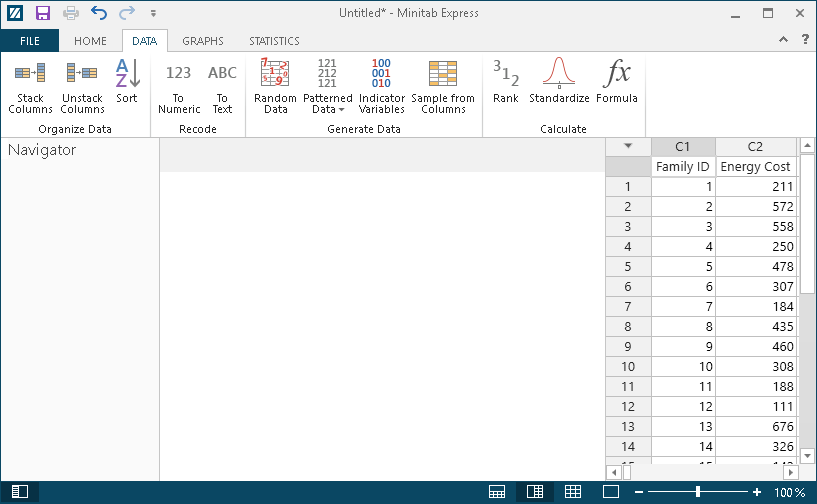
\includegraphics[scale=0.75]{minitab.png}
    \caption{Minitab - Visão geral}
    \label{fig:minitaboverview}
\end{figure}


É possível ainda gerar um conjunto de números aleatórios, com base em alguns parâmetros pré-definidos, através da opção \textit{Random Data} como exibido na Figura~\ref{fig:aleatorios}. Dentre os parâmetros, a média, o desvio padrão e a distribuição (Normal, Poisson, Weibull, dentre outras).

\begin{figure}[!h]
    \centering
    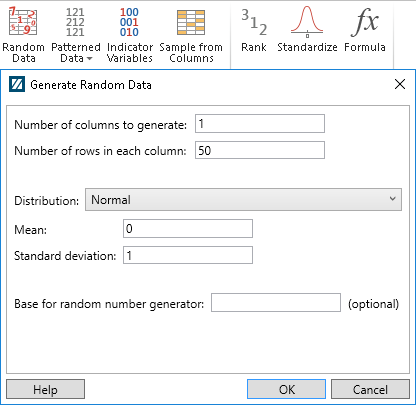
\includegraphics[scale=0.75]{aleatorios.png}
    \caption{Geração de números aleatórios}
    \label{fig:aleatorios}
\end{figure}

\newpage 

A partir da base de dados, é possível, através da opção \textit{Describe $>$ Descriptive Statistics}, ver um resumo estatístico dessa base. Na Figura~\ref{fig:descritiva} é exibido a opção no software, bem como os resultados da base utilizada de consumo energético.

\begin{figure}[!h]
    \centering
    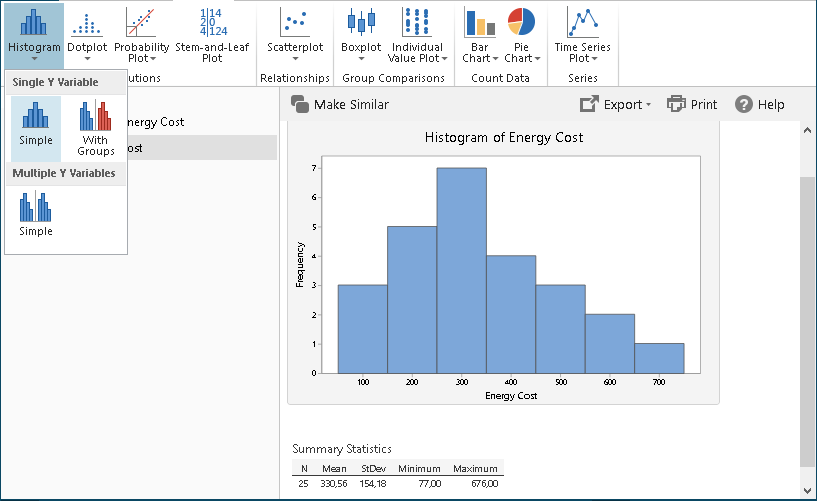
\includegraphics[scale=0.75]{descritiva.png}
    \caption{Medidas descritivas de variáveis quantitativas}
    \label{fig:descritiva}
\end{figure}

Também é possível gerar uma série de gráficos distintos no âmbito de estatística descritiva, para análises. Como exemplo, o Histograma, gerado através da opção \textit{Histogram $>$ Simple}. Na Figura~\ref{fig:historgama} é exibido a opção no software, bem como o histograma gerado.

\begin{figure}[!h]
    \centering
    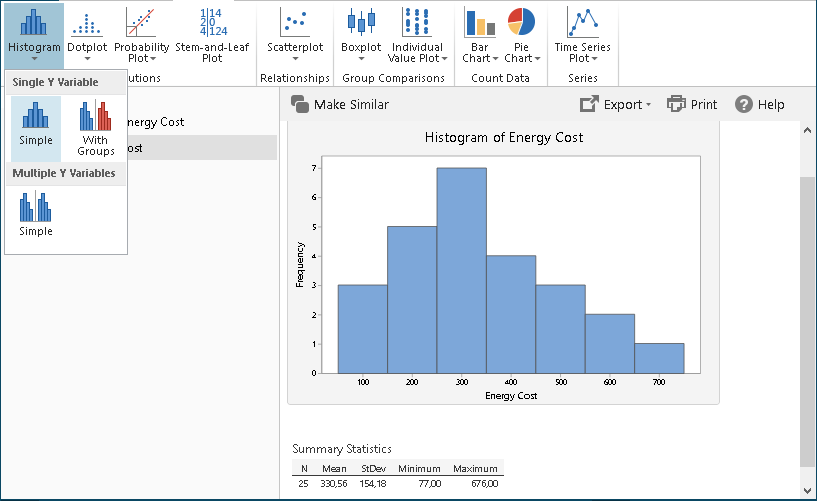
\includegraphics[scale=0.75]{histograma.png}
    \caption{Histograma}
    \label{fig:histograma}
\end{figure}

Da mesma forma, o gráfico BoxPlot é exibido na Figura~\ref{fig:boxplot}. Esse gráfico pode ser gerado através da opção \textit{Boxplot $>$ Simple}.

\begin{figure}[!h]
    \centering
    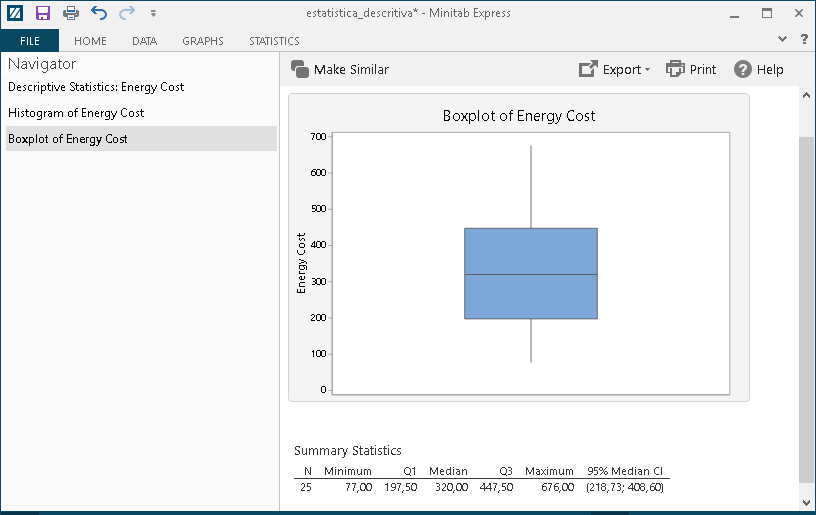
\includegraphics[scale=0.75]{boxplot.png}
    \caption{BoxPlot}
    \label{fig:boxplot}
\end{figure}

Por fim, é possível fazer a análise da distribuição de probabilidades, de maneira a identificar se o conjunto de dados segue uma distribuição Normal. A Figura~\ref{fig:probanalises} demonstra essa análise no \emph{Minitab}, acionada através da opção \textit{Normality Test}.

\begin{figure}[!h]
    \centering
    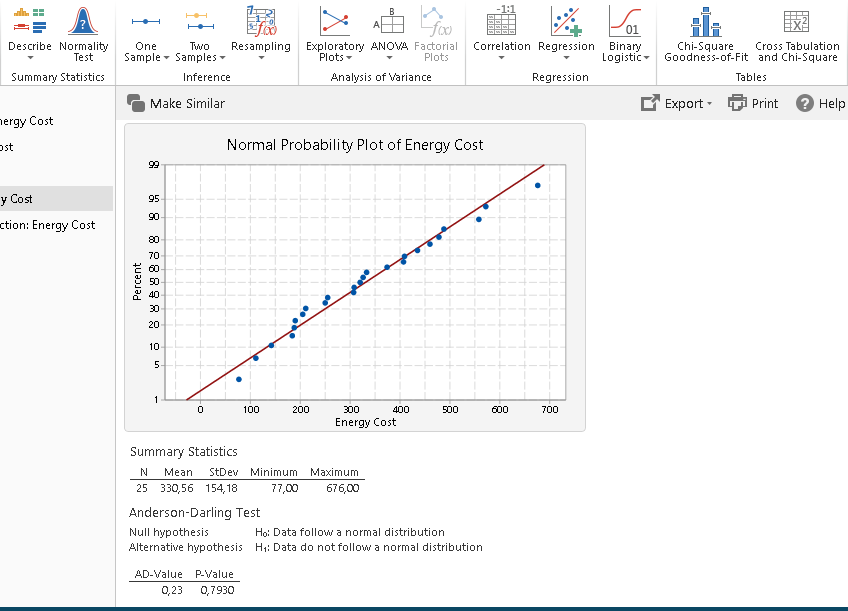
\includegraphics[scale=0.75]{probanalise.png}
    \caption{Teste de normalidade}
    \label{fig:probanalises}
\end{figure}

Nesta análise, são exibidos os resultados do teste de Anderson Darling, com as variáveis \emph{AD-value} e \emph{P-value}. Para análises mais completas, considerando outras distribuições, é necessário utilizar a versão completa do \emph{Minitab}, disponível para compra.



\section{Inferência Estatística}

Alguns testes de hipóteses, no contexto de inferência estatística, são apresentados neste capítulo. Foi realizada a implementação de algumas funções, usando apenas a linguagem R, considerada pelo grupo a mais adequada para tais fins.

\begin{rcode}{Inferência Estatística}
#----- Teste de hipotese - Teste para a Média com Variancia desconhecida
x <- c(19.8, 18.5, 17.6, 16.7, 15.8, 15.4, 14.1, 13.6,
     + 11.9, 11.4, 11.4, 8.8, 7.5, 15.4, 15.4, 19.5,
     + 14.9, 12.7, 11.9, 11.4, 10.1, 7.9)
x
t.test(x, alternative="greater", mu=10, conf.level=0.95)


#----- Teste de hipotese - Teste para a Variância de uma população normal
nam <- 20 #n = tamanho da amostra
varS <- 0.0153 #varS = variância amostral
sig0 <- 0.01 #sig0 = valor de variância testada
alfa <- 0.05 #alfa = significância do teste
quicalc = (nam-1) * varS / sig0
quicalc


#Funcao que testa uma variancia
onevartest <- function(varS, nam, sig0, alfa, tail){
  quicalc <- (nam-1)*varS/sig0; #estatística de teste
  #Testes unilaterais apenas
  if(tail==0){ #intervalo superior
    #pvalor do teste
    pvalor <- pchisq(q=quicalc,df=nam-1, lower.tail = F)
    Intervalo <- ((nam-1)*varS)/(qchisq(p=alfa,df=nam-1, lower.tail=F))
    print("P-Valor e Valor crítico do intervalo superior")
  }else{ #intervalo inferior
    #pvalor do teste
    pvalor <- pchisq(q=quicalc,df=nam-1, lower.tail = T);
    Intervalo <- ((nam-1)*varS)/(qchisq(p=alfa,df=nam-1, lower.tail=T))
    print("P-Valor e Valor crítico do intervalo inferior")
  }
  return(list(c("Pvalor =", pvalor),c("Intervalo = ", Intervalo)))
}
onevartest(varS, nam, sig0, alfa, 0)


#----- Teste para uma Proporção Binomial
x <- matrix(c(4,196),1,2)
x
prop.test(x,p=0.06,alternative="less",conf.level=0.97)


#----- Testes de Duas amostras para a diferença de duas médias com variâncias desconhecidas e diferentes
x <- c(91.50, 94.18, 92.18, 95.39,91.79,89.07,94.72,89.21)
y <- c(89.19,90.95,90.46,93.21,97.19,97.04,91.07,92.75)
x
y
t.test(x,y,alternative="two.sided",mu=0)


#----- Teste para as variâncias de duas populações normais
x <- rnorm(11, sd=5.1)
y <- rnorm(16, sd=4.7)
x
y
var.test(x,y,ratio=1,alternative="t",conf.level=0.9)

#----- Teste para duas proporções

X <- c(110,33)
Y <- c(201299, 200745)
X
Y
prop.test(X,Y,alternative="t")
prop.test(X,Y,alternative="t",conf.level=0.99) # Com a confiança
\end{rcode}


\section{ANOVA e MANOVA}

Neste capítulo exibe-se, também apenas em linguagem R, implementações dos métodos estatísticos ANOVA e MANOVA, para análise de variância de amostras. Implementações específicas também estão nos arquivos que acompanham este documento.

\begin{rcode}{ANOVA}
# Iniciando alguns dados para exemplo
data <- read.table(header=TRUE, text='
 subject sex   age before after
                   1   F   old    9.5   7.1
                   2   M   old   10.3  11.0
                   3   M   old    7.5   5.8
                   4   F   old   12.4   8.8
                   5   M   old   10.2   8.6
                   6   M   old   11.0   8.0
                   7   M young    9.1   3.0
                   8   F young    7.9   5.2
                   9   F   old    6.6   3.4
                   10   M young    7.7   4.0
                   11   M young    9.4   5.3
                   12   M   old   11.6  11.3
                   13   M young    9.9   4.6
                   14   F young    8.6   6.4
                   15   F young   14.3  13.5
                   16   F   old    9.2   4.7
                   17   M young    9.8   5.1
                   18   F   old    9.9   7.3
                   19   F young   13.0   9.5
                   20   M young   10.2   5.4
                   21   M young    9.0   3.7
                   22   F young    7.9   6.2
                   23   M   old   10.1  10.0
                   24   M young    9.0   1.7
                   25   M young    8.6   2.9
                   26   M young    9.4   3.2
                   27   M young    9.7   4.7
                   28   M young    9.3   4.9
                   29   F young   10.7   9.8
                   30   M   old    9.3   9.4
                   ')
                   
# ANOVA com 1 caminho de classificação
aov1 <- aov(before ~ sex, data=data)
summary(aov1)
# Exibe as médias           
model.tables(aov1, "means")

# ANOVA com 2 caminhos
aov2 <- aov(after ~ sex*age, data=data)
aov2 <- aov(after ~ sex + age + sex:age, data=data)
summary(aov2)
# Exibe as médias
model.tables(aov2, "means")

\end{rcode}

\begin{rcode}{MANOVA}
# Iniciando alguns dados para exemplo e importanto bibliotecas
wants <- c("car", "mvtnorm")
has   <- wants %in% rownames(installed.packages())
if(any(!has)) install.packages(wants[!has])
set.seed(123)
P     <- 3
Nj    <- c(15, 25, 20)
Sigma <- matrix(c(16,-2, -2,9), byrow=TRUE, ncol=2)
mu11  <- c(-4,  4)
mu21  <- c( 3,  3)
mu31  <- c( 1, -1)
library(mvtnorm)
Y11 <- round(rmvnorm(Nj[1], mean=mu11, sigma=Sigma))
Y21 <- round(rmvnorm(Nj[2], mean=mu21, sigma=Sigma))
Y31 <- round(rmvnorm(Nj[3], mean=mu31, sigma=Sigma))
dfMan1 <- data.frame(Y =rbind(Y11, Y21, Y31),
                     IV=factor(rep(1:P, Nj)))

# Análise simples usando MANOVA
manRes1 <- manova(cbind(Y.1, Y.2) ~ IV, data=dfMan1)
summary(manRes1, test="Wilks")
summary(manRes1, test="Roy")
summary(manRes1, test="Pillai")
summary(manRes1, test="Hotelling-Lawley")

# Usando MANOVA com 3 variáveis dependentes
Y <- cbind(y1,y2,y3)
fit <- manova(Y ~ A*B)
summary(fit, test="Pillai")


# Para MANOVA de 2 caminhos, vamos instanciar mais dados de teste
Q    <- 2
mu12 <- c(-1,  4)
mu22 <- c( 4,  8)
mu32 <- c( 4,  0)
library(mvtnorm)
Y12  <- round(rmvnorm(Nj[1], mean=mu12, sigma=Sigma))
Y22  <- round(rmvnorm(Nj[2], mean=mu22, sigma=Sigma))
Y32  <- round(rmvnorm(Nj[3], mean=mu32, sigma=Sigma))
dfMan2 <- data.frame(Y <- rbind(Y11, Y21, Y31, Y12, Y22, Y32),
                     IV1 <- factor(rep(rep(1:P, Nj), Q)),
                     IV2 <- factor(rep(1:Q, each=sum(Nj))))

# Usando a técnica com 2 caminhos
manRes2 <- manova(cbind(Y.1, Y.2) ~ IV1*IV2, data=dfMan2)
summary(manRes2, test="Pillai")
summary(manRes2, test="Wilks")
summary(manRes2, test="Roy")
summary(manRes2, test="Hotelling-Lawley")
\end{rcode}


\section{Considerações sobre este documento}

Os códigos aqui apresentados utilizaram base de dados de teste, mas podem ser facilmente adaptados para contemplar dados reais (basta mudar as matrizes ou conjuntos inicializados nos códigos).

A seguir, uma lista de arquivos que acompanham este documento, que podem ser usados em futuras implementações:

\begin{itemize}
    \item  1\_matrizes.py
    \item  1\_Matrizes.R
    \item  2\_Espacos\_Subespacos.py
    \item  2\_Espacos\_Subespacos.R
    \item  3\_PCA\_AnáliseFatorial\_SVD.py
    \item  3\_PCA\_AnáliseFatorial\_SVD.R
    \item  4\_RegressaoLinear\_Simples\_Multivariavel.py
    \item  4\_RegressaoLinear\_Simples\_Multivariavel.R
    \item  5\_estatistica\_descritiva.mpjx
    \item  6\_InferenciaEstatistica.R
    \item  7\_ANOVA\_MANOVA.R
    \item  metodos\_quantitativos.tex
\end{itemize}

Os arquivos com extensão \emph{.R}, são implementações em linguagem R, enquanto aqueles com extensão \emph{.py}, são implementações em Python. Os arquivos com extensão \emph{.mpjx} são arquivos de projeto do \emph{Minitab Express}. Também acompanha o código fonte deste documento.

\end{document}
